\Section{Производная}

\begin{definition}
	Пусть $ f : <a, b> \rightarrow \R $ \\
	f называется дифференцируемой в $ x_0 \in <a, b> $ \\
	если $ \exists k \in \R $ \\
	$ f(x) = f(x_0) + k(x - x_0) + o(x - x_0) $ при $ x \rightarrow x_0 $\\
	k - производная f в точке $ x_0 $
	\begin{lemma}
		Если f дифф в $ x_0 $ то $ f'(x_0) $ корректно определена 
		\begin{proof}
			$ f(x) = f(x_0) + k(x - x_0) + o(x - x_0) $ \\
			$ = f(x_0) + \tilde{k}(x - x_0) + o(x - x_0) $ \\
			$ \Rightarrow k(x-x_0) + o(x-x_0) = \tilde{k} (x -x_0) + o(x-x_0) $\\
			$ \Rightarrow k+\dfrac{o(x-x_0)}{x - x_0} = \tilde{k} + \dfrac{o(x-x_0)}{x-x_0} $ 
		\end{proof}$ \lim\lim\limits_{y \rightarrow y_0} g(y) = A $\\
	\end{lemma}
\end{definition}
\begin{definition}
	Произв $ f<a,b> \rightarrow \R $ в $ x_o \in <a,b> $ \\
	наз $ \lim\limits_{x \rightarrow x_0} \dfrac{f(x) - f(x_0)}{x - x_0} = f'(x_0) $ \\
	Если $ f'(x_0) \in \R$, то дифф 
\end{definition}

Предложение. Пусть $ f : <a, b> \rightarrow \R, x_0 \in <a, b> $ Тогда f дифф-ма в $x_0$ если и только если существует ф-ция $ \phi : <a,b> \rightarrow \R $ непрерывная в $x_0$ т.ч. $ f(x) - f(x_0) = \phi(x) (x-x_0), x \in <a,b> $ \\
$ f'(x_0) = \phi(x_0) $\\
\begin{proof} 
	$\Rightarrow$ предположим $ \phi(x) = \left\{ \begin{array}{ll}
		 \dfrac{f(x) - f(x_0)}{x - x_0}, x \neq x_0 \\
		 f'(x_0)
	\end{array} \right. $ \\
	Опр. 2 $ \phi(x) \rightarrow_{x - x_0} f'(x_0) = \phi(x_0) $\\
	То $\phi$ непрерывна в $x_0$ \\
	$\Leftarrow \phi$ непрерывна в $ x_0 \begin{array}{l} \Leftrightarrow \phi(x) \xrightarrow[{x - x_0}]{} \phi(x_0) \\
	\Leftrightarrow \phi(x)  = \phi(x_0) + o(1)_{\text{при} \ x \rightarrow x_0} \end{array} $ \\
	$ f(x) - f(x_0) = \phi(x_0) (x - x_0) + o(x-x_0) \Rightarrow f $ дифференци в $ x_0 $ и $phi(x_0) = f'(x_0) $    
\end{proof} 

\begin{definition}
	Говорят, что $ f'(x_0) = +\infty (-\infty) $, если \\
	$ \lim\limits_{x \rightarrow x_0} \dfrac{f(x) - f(x_0)}{x - x_0} =  +\infty (-\infty) $
\end{definition}

\begin{example}
	$ f(x) = \sqrt[3]{x}, x \in \R $ \\
	$ \lim\limits_{x \rightarrow 0} \dfrac{\sqrt[3]{x}}{x} =  \lim\limits_{x \rightarrow 0} \dfrac{1}{x^{2/3}} = +\infty $ \\
	Т.е. $ f'(x) = +\infty $ 
\end{example}

\begin{definition}
	$ f_+' (x_0) = \lim\limits_{x \rightarrow x_0+} \dfrac{f(x) - f(x_0)}{x - x_0} $ - правая производная \\
	$ f_-' (x_0) = \lim\limits_{x \rightarrow x_0-} \dfrac{f(x) - f(x_0)}{x - x_0} $ - левая производная \\
\end{definition}

Очевидно, пусть $ x_0 \in (a, b) $ \\ %pic1@
Тогда  $ \exists f'(x_0) \Leftrightarrow \left\{ \begin{array}{ll}
	\exists f_+' (x_0) \\
	\exists f_-' (x_0) \\
	f_+' (x_0) = f_-' (x_0) 
\end{array} \right. $
\begin{example}
	1. $ f(x) = x^2 $ \\
	$ f(x) - f(x_0) = x^2 - x_0^2 = (x-x_0)(x+x_0) $ \\
	$  \dfrac{f(x) - f(x_0)}{x - x_0} =_{x \neq x_0} x + x_0 \rightarrow_{x \rightarrow x_0} 2x_0  $\\
	$ f'(x_0) = 2x_0 $ \\
	2. $ f(x) = \sin(x) $ \\
	$ \sin(x) = \sin(x_0 + (x - x_0))  = \sin x_0 + \cos(x - x_0) + \cos(x_0) \sin(x-x_0) $ \\
	$ f(x) - f(x_0) = \underbrace{\sin(x_0) \cdot (\cos(x-x_0) - 1)}_{o(x-x_0)} + cos(x_0) (x- x_0) + o(x-x_0)  = \cos x_0 (x - x_0) + o(x - x_0) $ \\
	$ f'(x) = cos(x_0) $ 
\end{example}

\begin{properties}
	f - дифф-ма в $x_0 \Rightarrow f \ $ непрерывна в $x_0 $ \\
	$ f(x) = f(x_0) + \phi(x_0) (x - x_0), \phi $ непрерывна в $x_0 \Rightarrow $ f непрерывна в $x_0$ \\
	\begin{example}
		1. $ f(x) = |x| $ \\
		$ \dfrac{f(x) - 0}{x - 0} = \left\{ \right. $ \\
		$ f_+' (0) = 1, f_-' (0) = -1 $ \\
		2. $ f(x \neq 0) = x + \sin \dfrac{1}{x}, f(0) = 0, \lim\limits_{x \rightarrow 0} f(x) = 0 \Rightarrow f  $ непрерывна в 0 \\
		$ \dfrac{f(x) - f(0)}{x-0} = \dfrac{x \sin \dfrac{1}{x}}{x} =_{x>0} \sin \dfrac{1}{x} (x_{\pi} = \dfrac{1}{\pi n}, f(x_{\pi}) = 0, \tilde{x_{\pi}} =  \dfrac{1}{\pi n + \frac{\pi}{2}}, f(  \tilde{x_{\pi}} ) = 1  ) $ не имеет предела
	\end{example}   
\end{properties}


\Subsection{Физический и геометрический смысл производной}

$ x = f(t) $ \\
$ \dfrac{f(t) - f(t_0)}{t - t_0} $ - средняя скорость \\
$ \lim\limits_{x \rightarrow x_0} \dfrac{f(x) - f(x_0)}{x - x_0} = v(t_0) = f'(t_0) $ \\
\begin{center}
	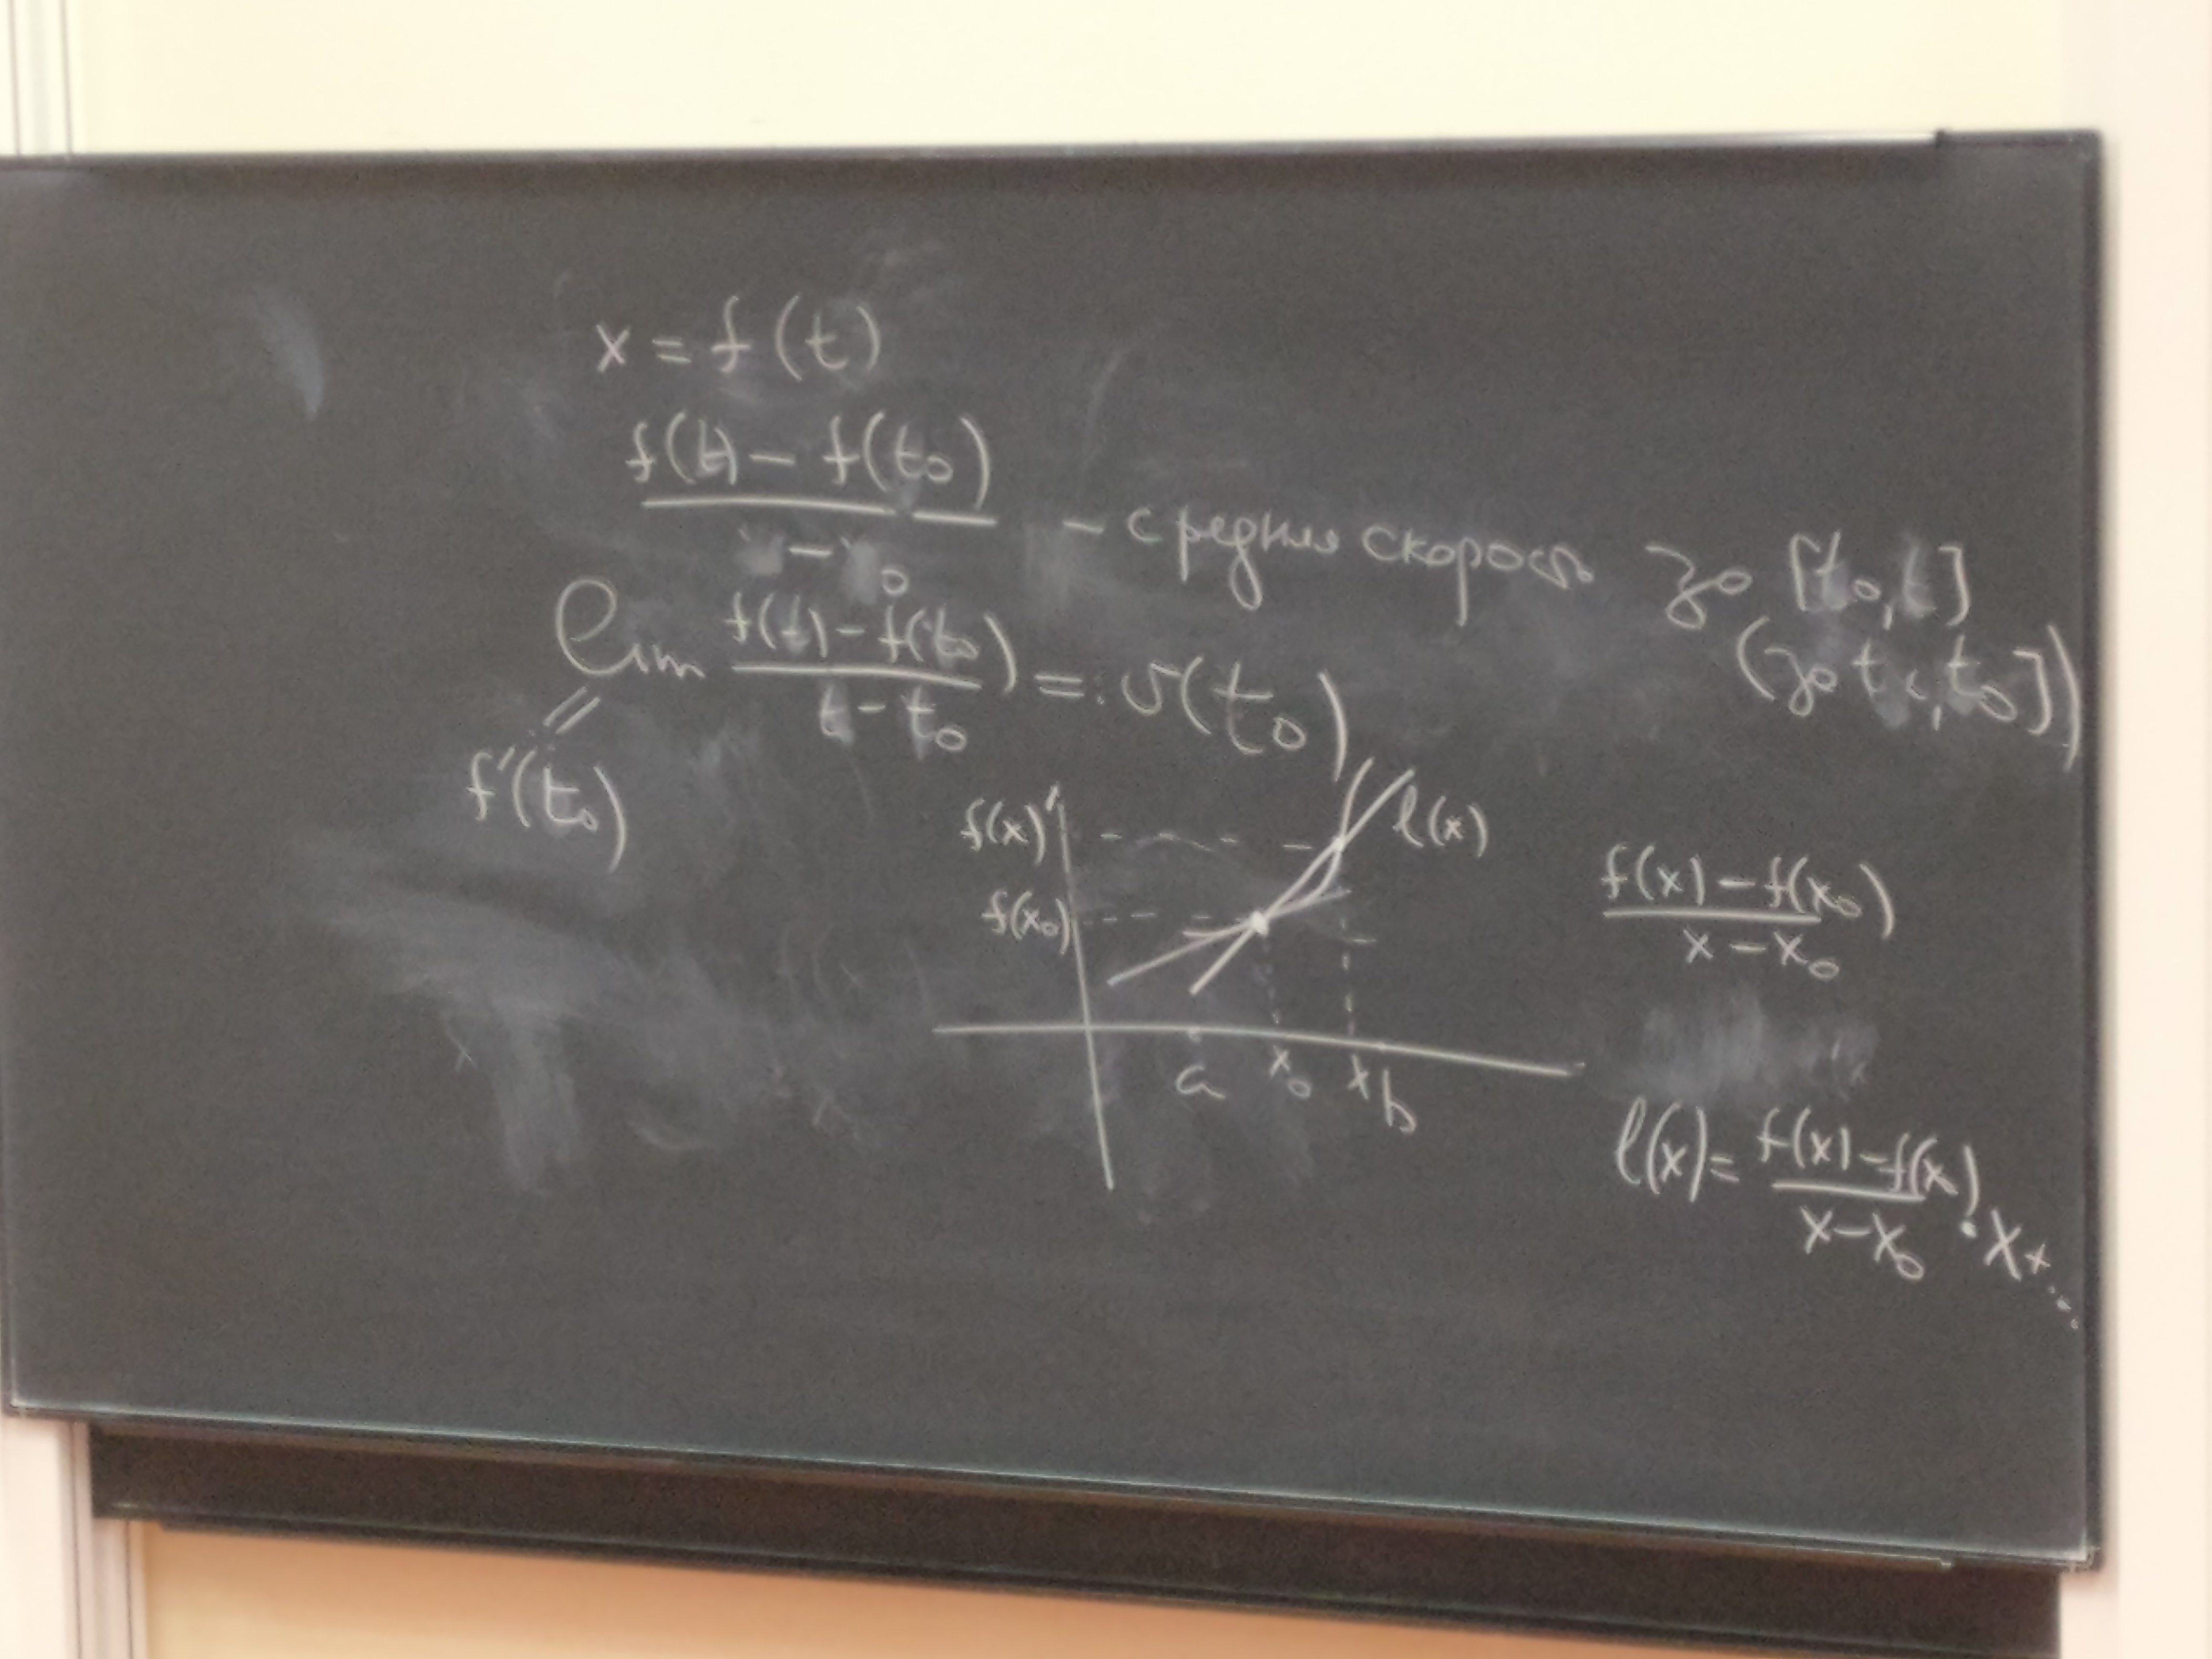
\includegraphics[width=0.9\linewidth]{IMG_20181119_124128}
\end{center}

%pic2@

\Subsection{Вычисление производных}

Предложение: пусть $ f, g < a, b> \rightarrow \R, x_0 \in <a,b>, f,g \text{дифф-мы в} x_0  $ \\
1. $ (\alpha f + \beta g)'(x_0) = \alpha f'(x_0) + \beta g'(x_0), \alpha, \beta \in \R  $ \\
2.$ (fg)'(x_0) = f'(x_0) g(x_0) + f(x_0) g'(x_0) $ \\
3. $ g(x_0) \neq 0, \text{тогда} \left( \dfrac{f}{g} \right)' (x_0) = \dfrac{ f'(x_0) g(x_0) - f(x_0) g'(x_0)}{g(x_0)^2} $ \\
\begin{proof}
	1. $ \lim \dfrac{  \alpha (f(x) - f(x_0)) + \beta (g(x) - g(x_0))}{x - x_0} = \alpha f'(x_0) + \beta g'(x_0) $ \\
	2. $ f(x) g(x) - f(x_0) g(x_0)  = f(x) g(x) - f(x_0) g(x) + f(x_0) g(x) - f(x_0) g(x_0) = (f(x) - f(x_0)) g(x) + f(x_0) (g(x) - g(x_0))$\\
	$ \lim\limits_{x \rightarrow 0} \dfrac{f(x)g(x) - f(x_0) g(x_0) }{x-x_0} = \lim\limits_{x \rightarrow 0} ( \dfrac{f(x) - f(x_0)}{x-x_0} \cdot g(x) ) + f(x_0) \lim\limits_{x \rightarrow 0} \dfrac{g(x) - g(x_0)}{x - x_0} = f'(x_0) g(x_0) + f(x_0)g'(x_0) $ \\
	3. $ (\dfrac{1}{g})'(x_0) = \lim\limits_{x \rightarrow 0} \dfrac{\frac{1}{g(x)} - \frac{1}{g(x_0)}}{x - x_0} = \lim\limits_{x \rightarrow 0} \dfrac{g(x_0) - g(x)}{(x-x_0) \underbrace{g(x_0) g(x)}_{g(x_0)^2} } = -\dfrac{g'(x_0)}{g(x_0)^2} $ \\
	$ (\dfrac{f}{g})' (x_0) = (f \cdot \dfrac{1}{g})' (x_0) = \dfrac{ f'(x_0) g(x_0) - f(x_0) g'(x_0)}{g(x_0)^2} $ 
\end{proof}

\begin{consequence}
	Пусть $ f(x) = a_n x^n + ... + a_1 x + a_0 $ \\
	Тогда $ f'(x_0) = na_n x_0^{n-1} + ... + 2 a_2 x_0 + a_1 $ \\
	Проверим $ (x^n)' = nx^{n-1} $ \\
	Очевидно верно при n = 1 \\
	$  (x^n)' = (x^{n-1} x )' = (x^{n-1})' x + x^{n-1} x' $ \\
	$ = (n-1) x^{n-1} x x^{n-1} \cdot 1 = nx^{n-1} $   
\end{consequence}

Предложение \\
Пусть $ f : <a,b> \rightarrow \R, g : <c, d> \rightarrow \R $ \\
$ f $ дифф-ма в $ x_0 \in <a,b> $ \\
$ f(<a,b>) \in <c,d> $ \\
$ g \ \ \text{дифф-ма в} f(x_0) $ \\
Тогда $ g \circ f $ дифф-ма в $ x_0 $ \\
$ (g \circ f)' (x_0) = g'(f(x_0)) \cdot f'(x_0) $ \\
$ f(x) - f(x_0) =(x-x_0) \cdot \phi(x), \phi $ непрерывн в $x_0$ \\
$ g(y) - g(y_0) = (y - y_0) \cdot \psi (y), \psi $ непрерывн в $ y_0 $ \\
$ g(f(x)) - g(f(x_0)) = ( f(x) - f(x_0) ) \cdot \psi(f(x)) = (x-x_0) \cdot \phi(x) \cdot \psi(f(x)), x \in <a,b> $ \\
$ f(x) $ непр в x \\
$ \psi(f(x)) $ непр в x \\
$ g \circ f $ дифф в $ x_0$ \\
$ (g \circ f)'(x_0) = \phi(x_0) \cdot \psi(f(x_0)) = f'(x_0) \cdot g'(f(x_0)) $ \\

$ (\sin(x^2))' = \cos(x^2) \cdot 2x $

\begin{center}
	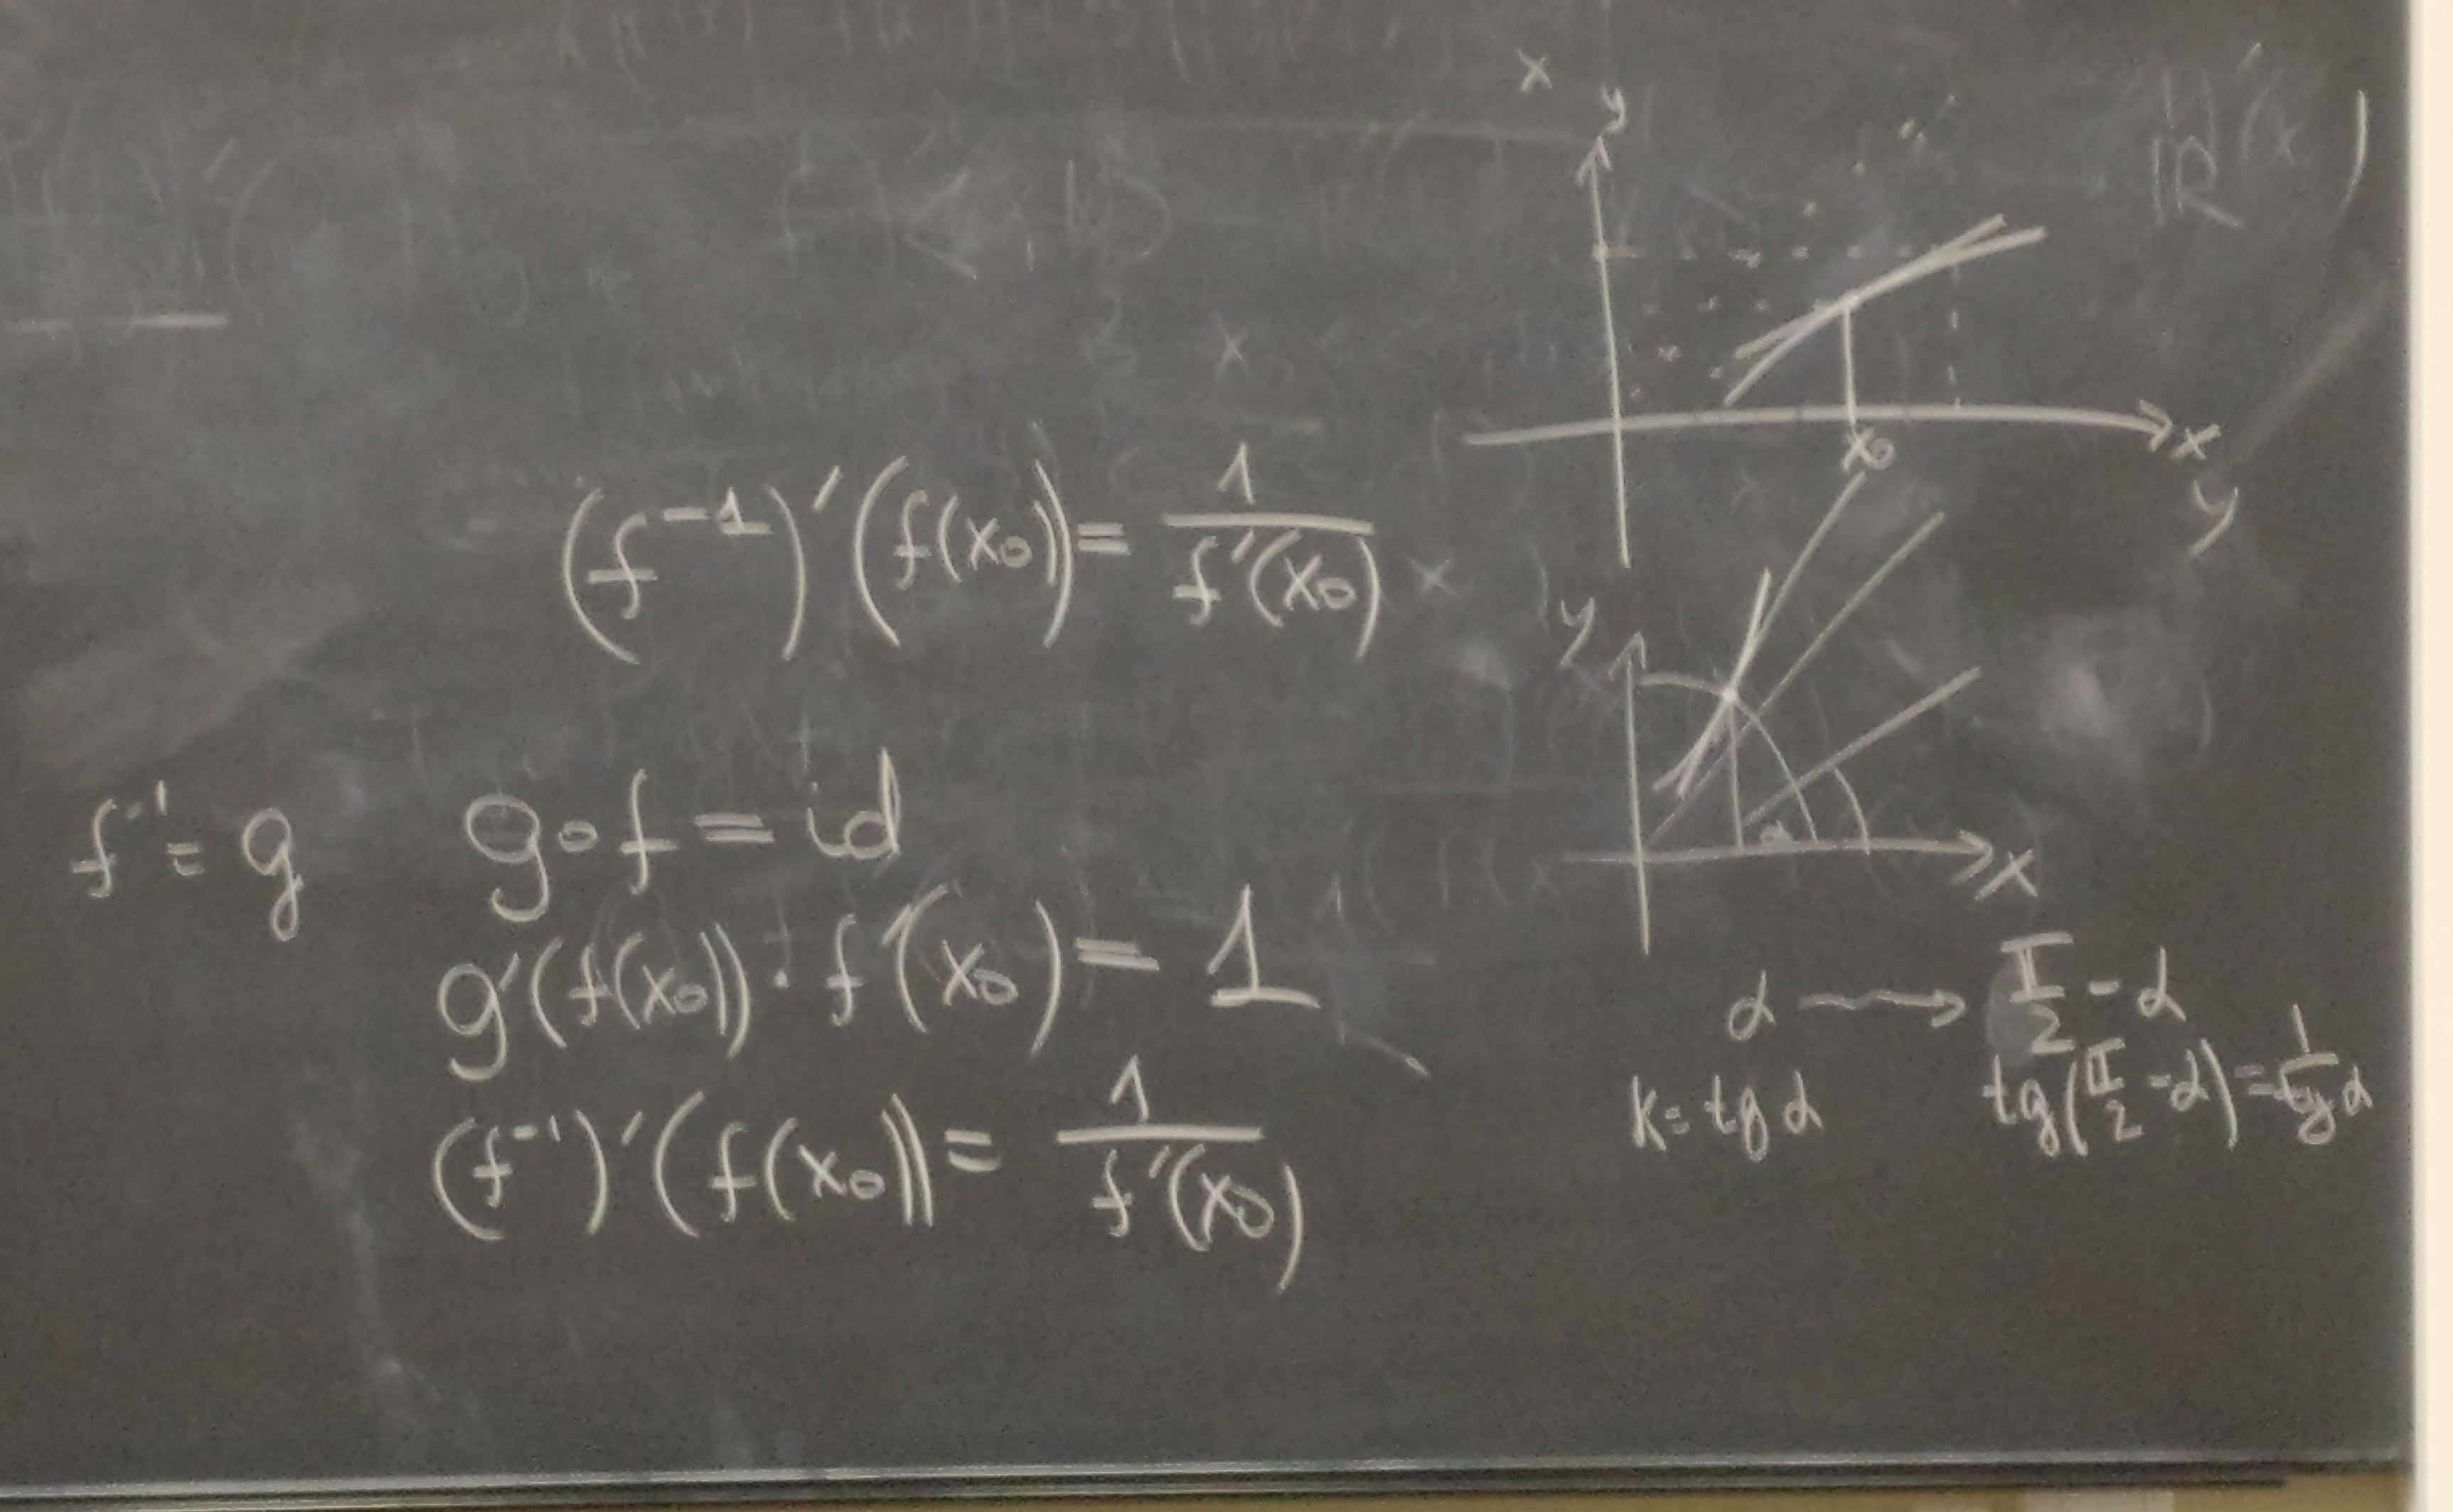
\includegraphics[width=0.9\linewidth]{IMG_20181119_133702}
\end{center}

$ f^{-1} = g $ \\
$ g \circ f = id $ \\
$ g'(f(x_0)) \cdot f'(x_0) = 1 $ \\
$ (f^{-1})' (f(x_0)) = \dfrac{1}{f'(x_0)} $\\

 






 